\documentclass[a4paper]{article}

%%%%%%%%%%%%%%%%%%%%%%%%%%%%%%%%%%%%%%%%%%%%%%
\usepackage[T1]{fontenc}
\usepackage{geometry}
\geometry{a4paper,left=1.5cm,right=1cm,top=1cm,bottom=1cm}

\usepackage{graphicx}
\usepackage[absolute,overlay]{textpos}
\usepackage{eso-pic}               % image de fond
\usepackage{fontawesome5}
\usepackage[hidelinks]{hyperref}
\usepackage{tikz}
\usepackage{xcolor}
\usepackage{enumitem}
\setlist{nosep,leftmargin=6mm}
\usepackage{times}                % même police que votre exemple
\usepackage{array} 
\usepackage{tabularx}
\usepackage{ragged2e}
\let\origcolorbox\colorbox    % sauvegarde
\renewcommand{\colorbox}[2]{#2}% neutralise le fond
%%%%%%%%%%%%%%%%%%%%%%%%%%%%%%%%%%%%%%%%%%%%%%
%\definecolor{texcolor}{HTML}{e2e8f0}
\providecolor{sidetext}{rgb}{1,1,1}
\definecolor{maincolor}{HTML}{ffffff}

%%%%%%%%%%%%%%%%%%%%%%%%%%%%%%%%%%%%%%%%%
% — Ne changez pas le nom : « background.jpg » doit être présent
\AddToShipoutPictureBG*{%
  
\includegraphics[width=\paperwidth,height=\paperheight]{background.jpg}%
}

%%%%%%%%%%%%%%%%%%%%%%%%%%%%%%%%%%%%%%%%%
\newcommand{\fullrule}{\hspace{-1.5cm}\rule{\paperwidth}{0.4pt}}
\newcommand{\cvsection}[1]{%
  \vspace{6pt}\textbf{\Large #1}\par\vspace{2pt}}
\newcommand{\cicon}[1]{%
  \tikz[baseline]{\draw[fill=white] (0,0.1) circle[radius=0.1cm];}~#1}

\setlength{\parindent}{0pt}
%\color{texcolor}
%%%%%%%%%%%%%%%%%%%%%%%%%%%%%%%%%%%%%%%%%%%%%%%%%%%%%%%%%%%%%%
\begin{document}
\color{white}
% ---------- Photo ------------------------------------------------
\begin{textblock*}{4cm}(0.2cm,0.3cm)
  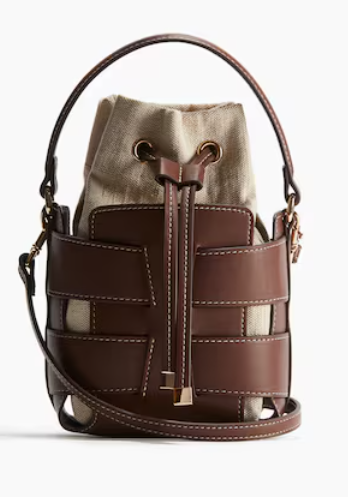
\includegraphics[width=2.5cm,clip,keepaspectratio]{990139eb0e804d108f14c2dc6eeafd1f.png}
\end{textblock*}

% ---------- En-tête ---------------------------------------------
\begin{center}
  {\fontsize{44pt}{24pt}\selectfont\bfseries Judikael Mourouvin}

  \bigskip
  {\Large Alternant en marketing digital \& support informatique}

  \bigskip\bigskip
  \faMapMarker~Route de COCOYER\ 97190 Gosier
  \quad\faEnvelope~\href{mailto:jkmou971@gmail.com}{jkmou971@gmail.com}

  \bigskip
  % Badge LinkedIn (retirez-le si inutile)
  \faPhone~ +590 0690 91 14 48
  \quad \faLinkedin\ \href{}{}
 

  \vspace{-0.3cm}
  \fullrule
\end{center}

% ---------- Profil ----------------------------------------------
\cvsection{Profil}

Passionné par l’informatique et le marketing digital, je maîtrise la configuration de postes, la maintenance et le diagnostic d’incidents. Mon année d’alternance à la DSI de la Mairie du Gosier m’a permis de conduire des projets numériques et de former les utilisateurs. Curieux et rigoureux, je souhaite désormais m’engager à plein temps pour accompagner le développement de vos solutions digitales. Mon sens du service et mon aisance technique constitueront de solides atouts pour votre équipe.

\medskip\fullrule

% ---------- Expérience ------------------------------------------
\cvsection{Expérience}
\hspace*{1.3cm}%

\colorbox{maincolor}{%
  \begin{minipage}{\linewidth}
    \textbf{Alternant en marketing digital} \\ Mairie du Gosier – DSI \\ 2023-2024
    \begin{itemize}
      \item Coordonné les projets numériques de la mairie, assurant leur déploiement dans les délais \item Analysé les besoins des agents et mis en place des solutions adaptées pour optimiser les processus \item Dispensé un support technique et des formations aux utilisateurs tout en contribuant à la stratégie digitale
    \end{itemize}
  \end{minipage}}

\vspace{3mm}


\colorbox{maincolor}{%
  \begin{minipage}{\linewidth}
    \textbf{Animateur de la zone informatique} \\ Pôle Emploi, Gosier \\ 2022-2023
    \begin{itemize}
      \item Assisté les usagers dans l’utilisation des services numériques de Pôle Emploi \item Configuré et maintenu les postes de travail de l’espace informatique pour garantir leur disponibilité \item Diagnostiqué et résolu les incidents matériels et logiciels, réduisant les interruptions de service
    \end{itemize}
  \end{minipage}}

\vspace{3mm}


\colorbox{maincolor}{%
  \begin{minipage}{\linewidth}
    \textbf{Stagiaire informaticien} \\ NUMERIKA, Baie-Mahault \\ 2020-2021
    \begin{itemize}
      \item Installé et configuré divers équipements informatiques pour les clients \item Réalisé la maintenance préventive et corrective du parc afin d’améliorer sa stabilité \item Assuré le support technique de première ligne, maintenant la continuité des opérations
    \end{itemize}
  \end{minipage}}

\medskip\fullrule

% ---------- Éducation -------------------------------------------
\cvsection{Éducation}
\hspace*{1.3cm}%

    \begin{tabularx}{\linewidth}{@{}c >{\RaggedRight\arraybackslash}X@{}}
    \textcolor{sidetext}{\faGraduationCap} &
    \textbf{Bachelor Marketing Digital} \\
    & CFA IUTS \\
    & \textit{2023-2024} \\
    \end{tabularx}
    \begin{itemize}[leftmargin=*]
  \item Apprentissage des leviers du marketing en ligne : SEO, SEA et réseaux sociaux
  \item Conception de stratégies digitales et analyse de performance
  \item Gestion de projets et utilisation d’outils de communication numérique
\end{itemize}
\vspace{3mm}

    \begin{tabularx}{\linewidth}{@{}c >{\RaggedRight\arraybackslash}X@{}}
    \textcolor{sidetext}{\faGraduationCap} &
    \textbf{BTS Systèmes Numériques option Informatique et Réseaux} \\
    & Lycée de Chevalier Saint Georges, Abymes \\
    & \textit{2019-2021} \\
    \end{tabularx}
    \begin{itemize}[leftmargin=*]
  \item Étude des architectures matérielles, systèmes et réseaux
  \item Développement et intégration de solutions logicielles embarquées
  \item Maintenance et sécurisation des infrastructures informatiques
\end{itemize}

\medskip\fullrule

% ---------- Compétences -----------------------------------------
\cvsection{Compétences}
\\
\hspace*{2.2cm}%
\begin{tabular}{@{}p{0.25\linewidth}p{0.18\linewidth}p{0.18\linewidth}p{0.18\linewidth}}\cicon Administration & \cicon Réseaux & \cicon Support & \cicon Maintenance \\
\cicon Configuration & \cicon Diagnostic & \cicon Marketing & \cicon Digital \\
\cicon Assistance & \cicon Formation & ~ & ~ \\\end{tabular}   % grille 3 lignes × 4 colonnes

\end{document}
